\section{Machine learning techniques and Related works}
\label{sec:techs}

In this section we summarize the machine learning techniques used and we present the main related works.

\subsection{Support Vector Regression (SVR)}

\TODO{Estoy seguro que los lectores van a solicitar reducir esto y
  dejar solo la referencia.  No hay nada nuevo en el resto del paper
  que requiera toda esta información, así que hay que resumirlo a nada
  más lo esencial. }


From the perspective of Support Vector Regression (SVR) the regression
function $y = f(s)$ for a given dataset $D=\{(s_i,y_i)\}_{i=1}^n$ is
represented as a linear function of the form \citep{Wei2013}:
\begin{equation*}
  f(s)=w^Ts+b
\end{equation*}
where $w$ and $b$ are respectively the weight vector and the intercept
of the model, and they are selected to find an \todofn{optimal}%
{optimal respecto a qué?.  Hay muchísimas posibilidades de optimalidad!}
%
fit to the data available in $D$ \review{in the sense of ...?}

For nonlinear cases, the $p$-dimensional input vectors are mapped by a
nonlinear function $\phi : R^p\rightarrow F$ onto a feature space
$F$.  After the nonlinear mapping, the regression function evolves to a
pervasive form:
\begin{equation*}
f(s)=w^T \phi (s)+b
\end{equation*}

In SVR the generalization ability is measured by the Euclidean norm of
$w$, and the empirical error is measured by the $\epsilon$-insensitive
loss function, given by \citep{Cristiani2005}

\TODO{si $l$ es una función, es función de qué, de $s$? $l(s)$? o de
  $y$? o de todos $l(y,s;\epsilon)$?}

\begin{equation*}
l= {\left| y - f(s) \right| }_{\epsilon } = 
\begin{cases}
   0 & {\left| y - f(s) \right| } \leq \epsilon \\
   \left| y - f(s) \right| - \epsilon & \text{otherwise}
\end{cases}
\end{equation*}
which ignores the error if the difference between the prediction value
and the actual value is smaller than $\epsilon$.
%
The $\epsilon$-insensitive loss function allows to find the
coefficients $w$ and $b$ by solving a convex optimization problem,
which balances the empirical error and the generalization ability.
%
Then, the optimization problem to identify the regression model can be
formulated as \citep{Wei2013}:
%
\begin{equation} 
\begin{aligned}
& \underset{}{\text{minimize}}
& & J(w,\xi_i , \xi_i^* ) = \frac{1}{2}   \Bigr| \Bigr| w \Bigr| \Bigr|^2 + C \sum_{i=1}^{n} (\xi_i , \xi_i^* )    \\
& \text{subject to}
& & \begin{array}{lcl} 
y_i - w^T \phi (s) - b  \leq \epsilon + \xi_i   \\
w^T \phi (s) + b - y_i \leq \epsilon + \xi_i^* & i= 1,2,...,n \\
\xi_i , \xi_i^* \geq 0  \\
\end{array}
\end{aligned}
\end{equation}  
where $C$ denotes the penalty parameter between empirical and
generalization errors, and $\xi_i , \xi_i^*$ are slack
variables. \figref{figura2} shows this situation.

\begin{figure}[h] 
 \centering
 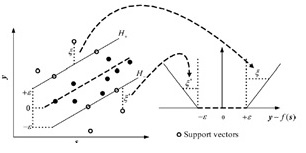
\includegraphics[scale=.9]{SVR}
 \caption{$\epsilon$-insensitive loss function \citep{Wei2013}.} 
 \label{figura2} 
\end{figure}
 
The solution of this optimization problem by the Lagrange method is given by:
\begin{equation*}
f(s) = w^T \phi (s) + b = \sum_{i=1}^{n} (\alpha_i - \alpha_i^*) K (s,s_i) + b
\end{equation*}
where $\alpha_i - \alpha_i^*$ are the Lagrange multipliers of the
optimization problem’s dual form and $K(s_i,s_j )$ is the kernel
function satisfying the Mercer condition, and holds:
\begin{equation*}
K(s_i,s_j ) = \big \langle  \phi(s_i) , \phi(s_j)  \big \rangle
\end{equation*}
Operations in the kernel function $K(s,s_i )$ are performed in the
input space rather than in the potentially high dimensional feature
space of $\phi$ \citep{Alonso2013}.

\subsection{Ordinary least squares regression}

This method fits a linear model with coefficients $w = (w_1,..,w_p)$
to minimize the residual sum of squares between the observed responses
in the dataset, and the responses predicted by the linear
approximation. Mathematically it solves a problem of the form
\citep{scikitlearn2011}:
$$\min_{w} \Bigr| \Bigr| Xw - y \Bigr| \Bigr|_2^2  $$
where $X$ denotes the features matrix.

According Pedregosa et al. \citep{scikitlearn2011}  the coefficient estimates for Ordinary Least Squares rely on the independence of the model terms. When terms are correlated and the columns of the design matrix $X$ have an approximate linear dependence, the design matrix becomes close to singular and as a result, the least-squares estimate becomes highly sensitive to random errors in the observed response, producing a large variance. This situation of multicollinearity can arise, for example, when data are collected without an experimental design.

\subsection{Ridge regression}
The ridge regression addresses some of the problems of ordinary least squares regression by imposing a penalty on the size of the coefficients. The ridge coefficients minimize a penalized residual sum of squares  \citep{scikitlearn2011}:

$$\min_{w} { \Bigr| \Bigr| Xw - y \Bigr| \Bigr|_2^2  + \alpha \Bigr| \Bigr| w \Bigr| \Bigr|_2^2 } $$

Here, $\alpha \ \textgreater \  0$ is a complexity parameter that controls the amount of shrinkage: the larger the value of $\alpha$, the greater the amount of shrinkage and thus the coefficients become more robust to collinearity.

\subsection{Elastic-Net regression}
Elastic-Net is a linear regression model trained with $L1$ and $L2$ prior as regularizer. This combination allows for learning a sparse model where few of the weights are non-zero like Lasso, while still maintaining the regularization properties of Ridge  \citep{scikitlearn2011}. The convex combination of $L1$ and $L2$ is controled by using the $l1_{ratio}$ parameter.

Elastic-Net is useful when there are multiple features which are correlated with one another. Lasso is likely to pick one of these at random, while elastic-net is likely to pick both.
A practical advantage of trading-off between Lasso and Ridge is it allows Elastic-Net to inherit some of Ridge’s stability under rotation. The objective function to minimize is \citep{scikitlearn2011}:

$$\min_{w} { \frac{1}{2n_{samples}} \Bigr| \Bigr| Xw - y \Bigr| \Bigr|_2^2  + \alpha \rho \Bigr| \Bigr| w \Bigr| \Bigr|_1 + \frac{\alpha (1- \rho)}{2} \Bigr| \Bigr| w \Bigr| \Bigr|_2^2 } $$

\subsection{Echo State Networks (ESN)}
Recurrent Neural Networks (RNN) are useful for temporal patterns, but when they are trained with backpropagation methods, they are very slow.  Echo State Network (ESN) is an alternative training method to solve that problem.  ESN is based on the observation that if a random RNN possesses certain algebraic properties, training only a linear readout from it is often sufficient to achieve excellent performance in practical applications \citep{Lukose2009}. 
For a given training input signal $u(n)  \in R^{N_u}$ a desired target output signal $y^{target}(n) \in R^{N_y}$
is known. Here $n = 1, . . . ,T$ is the discrete time and $T$ is the number of data points in the training dataset. The task is to learn a model with output $y(n) \in R^{N_y}$, where $y(n)$ matches $y^target(n)$ as well as possible, minimizing an error measure $E(y,y^target)$, and, more importantly, generalizes well to unseen data. The untrained RNN part of an ESN is called a dynamical reservoir, and the resulting states x(n) are termed echoes of its input history \citep{Lukose2012}. Finally, these signals are sent to an output layer as shown in the \figref{figura3}.
\begin{figure}[h] 
 \centering
 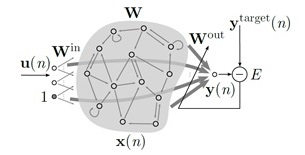
\includegraphics[scale=.9]{Reservorio}
 \caption{An echo state network \citep{Lukose2012}.} 
 \label{figura3} 
\end{figure}
 
The connections between the different elements of an Echo State Network have weights randomly generated. The weights of the internal connections of the reservoir $(W)$ as well as the weights of the input layer $(W_in)$, after being generated are set statically during all stages of implementation of the algorithm. The weights between the reservoir and the output layer $(W_out)$ are subject to changes of a supervised learning algorithm to correct the degree of error generated by the entire system \citep{Lukose2012}.
